\newpage

\section{فصل دهم}

یک عمل، توسط \lr{Agent} انجام می‌شود که در یک کلاس، تغییرات جدیدی را اعمال
می‌کند و می‌تواند بر \lr{State}های آن کلاس تاثیر بگذارد. به همین خاطر از
نمودار‌های کلاس \footnote{\lr{Class diagram}} استفاده می‌کنیم که به عنوان
ساختمان داده‌ای از \lr{State} را داشته باشیم، اما این نمودار با نمودار کلاس در
فاز طراحی متفاوت است که فاقد جزئیات می‌باشد. این کلاس فاقد بخش‌های زیر می‌باشد:

\begin{LTR}
    \begin{itemize}
        \item \lr{Encapsulaction}
        \item \lr{Methods (As class behaviors)}
        \item \lr{Abstraction}
    \end{itemize}
\end{LTR}

\subsection*{نکات}

\begin{itemize} 
    \item در واقعیت امر موارد بالا را طراح و معمار نرم‌افزار تعیین می‌کند که یک
    کلاس می‌تواند چه رفتار‌ها (عملکرد‌هایی) و قابلیت‌هایی داشته باشد.
    \item این کلاس‌ها، در حقیقت نمای کلی از کلاس‌های فضای مسئله هستند.
    \item فضا‌های راه‌حل مختص زمان طراحی نرم‌افزار هستند.
    \item نقاط را به صورت دنباله‌ای از مراحل به هم متصل می‌کنیم.
\end{itemize}

\subsection{اجزای سازنده کلاس در مرحله نیازمندی}

یک کلاس در مهندسی نیازمندی تنها موارد زیر را دارد:

\begin{enumerate}
    \item ویژگی، استیت‌ها یا \lr{Attributes}
    \item \lr{Annotation}: تعریف یک کلاس
    \item روابط کلاس‌ها:
    \begin{enumerate}
        \item \lr{Association} یا انجمنی
        \item \lr{Inheritance} یا وراثت
        \item \lr{Composition} یا ترکیب
        \item \lr{Aggregation} یا تجمیع
        \item \lr{Multiplicity} یا تعدد
    \end{enumerate}
\end{enumerate}

\subsection{روابط بین کلاس‌ها}

یکی از مهم‌ترین بخش‌های کلاس‌ها را روابط بین آن‌ها تشکیل می‌دهند که تعریف هر
کدام به شکل زیر می‌باشد:

\subsubsection{\lr{Association} یا انجمنی}

در این نوع ارتباط، رابطه بین کلاس‌ها را از طریق فعل نمایش می‌دهیم.

@startuml trainBlock
class Train {
  + doorState
  + acceleration
  + speed
}

class Block { }

Train -- Block: "On"
@enduml

@startuml trainPlatform
class Train {
  + doorState
  + acceleration
  + speed
}

class Platform { }

Train -- Platform: "At"
@enduml

@startuml patronBookcopy
class Patron {
 + id: string
 + phone: string
 + fullname: string
}

class BookCopy {  }

Patron -- BookCopy: "Loan"
@enduml

% \begin{figure}[H]
%     \centering
%     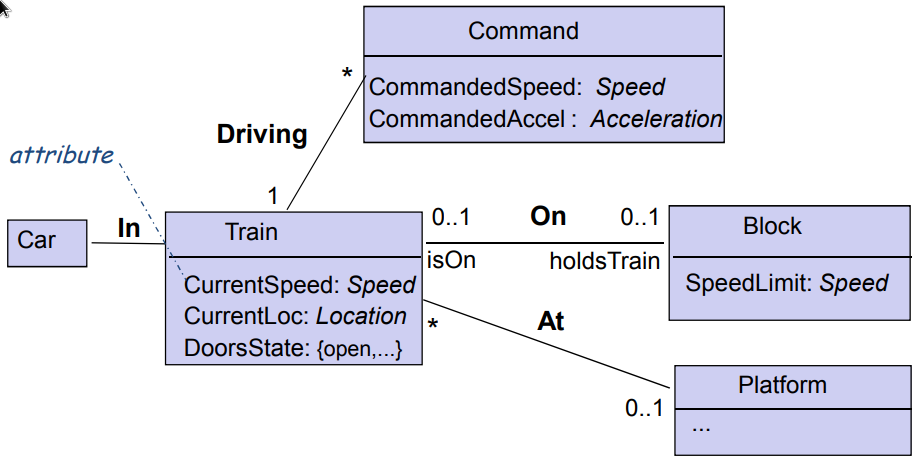
\includegraphics[width=0.7\textwidth]{images/association_diagram.png}
%     \caption{\lr{Entities, Associations, Attributes in UML}}
% \end{figure}

% \begin{figure}[H]
%     \centering
%     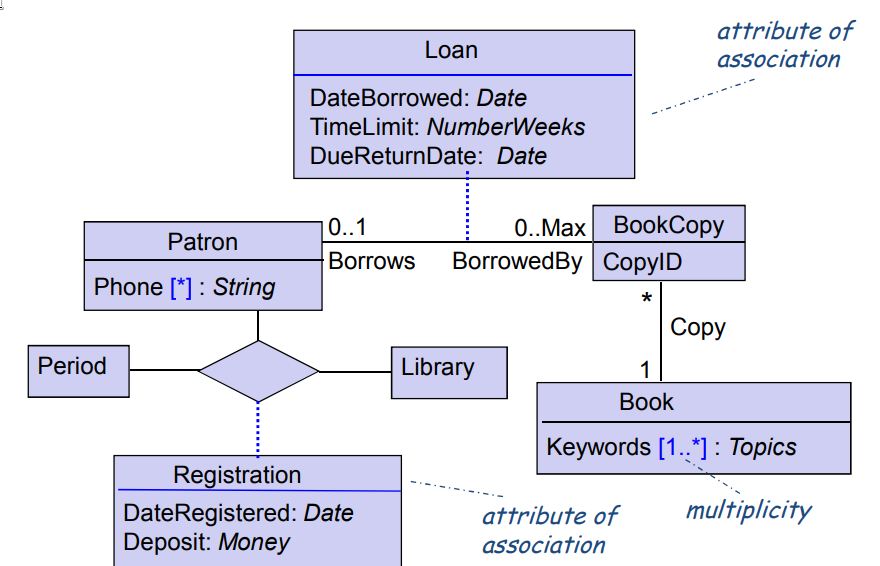
\includegraphics[width=0.7\textwidth]{images/association_diagram_2.png}
%     \caption{\lr{Entities, Associations, Attributes more details in UML}}
% \end{figure}

\subsubsection{\lr{Inheritance} یا وراثت}

در این نوع از روابط، رابطه بین کلاس‌ها به صورت والد و فرزندی می‌باشد که فرزندان
ممکن است برخی یا همه صفات کلاس والد را به ارث برده باشند یا برخی کلاس‌ها با توجه
به نیاز خود، صفات محدودتری را به ارث برده باشند. معمولاً این کلاس در قدم‌های
ابتدایی مسئله دیده می‌شود.

برای مثال، یک کتاب، یک محتوای آموزشی می‌باشد. همچنین یک فیلم نیز یک محتوای
آموزشی. در این مثال محتوای آموزشی را به عنوان کلاس والد در نظر می‌گیریم که
می‌تواند به شکل‌های مختلفی مانند فیلم یا کتاب نوشتاری ارائه شوند.

\subsubsection{\lr{Composition} یا ترکیب}

در این نوع رابطه، گاهی یک شئ مستقل نداریم، (برای مثال شئ‌ای به نام ماشین نداریم)
هویت یک کلاس با مهم‌ترین بخش‌های آن مشخص می‌شود. برای مثال یک پیام تشکیل شده از
۳ بخش مهم، بدنه، سرتیتر، فوتر. اگر این ۳ بخش به صورت یکپارچه در کنار هم باشند
ساختار اصلی پیام را تشکیل می‌دهند زیرا هر بخش به عنوان جز مستقل نمی‌باشد بلکه
رابطه کل به جز می‌باشد.

برای مثال \lr{Session} یک دستگاه \lr{ATM} رابطه کل به جز در خصوص واریزی‌ها و
تراکنش‌ها می‌باشد. زمانی که \lr{Session} یک کاربر (با خروج کارت) به پایان رسید،
\lr{Session} کاربر قبلی بایستی از بین برود \footnote{\lr{Distory}}. در حقیقت
باید ببینیم که نیاز سیستم چیست و چه زمانی اتفاق می‌افتد. این موارد به صورت
قانونی نیست بلکه به صورت تصمیم می‌باشد. در حقیقت در این بخش می‌تواند از افراد
خبره و متخصص این بخش استفاده کرد. حیات جز به حیات کل سیستم وابسته می‌باشد.

\subsubsection{\lr{Aggrigation} یا تجمیع}

این رابطه مشابه رابطه ترکیبی یا \lr{Composition} می‌باشد با این تفاوت که در
تجمیع بیان می‌شود که اگر کل از بین برود، اجزا باز هم باقی می‌ماند.

\begin{figure}[H]
    \centering
    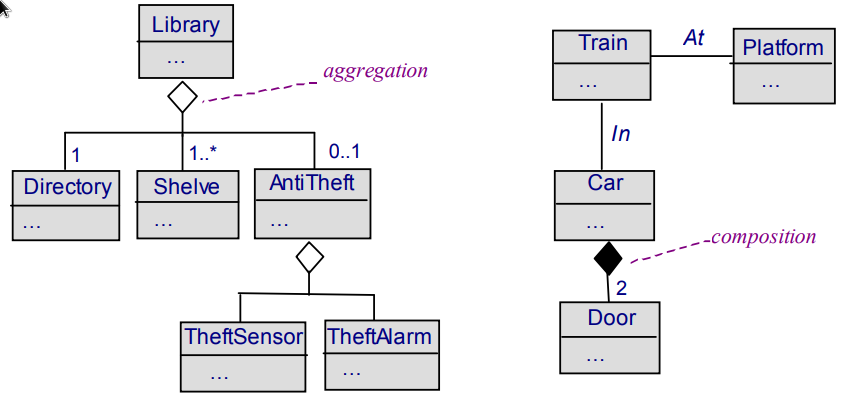
\includegraphics[width=0.7\textwidth]{images/aggregation_relation.png}
    \caption{\lr{Object aggregation: example}}
\end{figure}

\subsubsection{\lr{Multiplicity} یا تعدد}

در این رابطه، هر نمونه‌ای از یک کلاس با تعدادی از نمونه‌های کلاس دیگر ارتباط
دارند.

\begin{LTR}
    \begin{itemize}
        \item $[0..x]$: Optional attribute
        \item $[x..*]$: Attribute value = Set of values
        \item $[1..1]$: Mandatory attribute, single value: by default, omitted
        \item e.g. $phoneNumber$ $[0..*]$: String, optional possibly multiple
        values
    \end{itemize}
\end{LTR}

بر اساس دو اصل کار می‌کند، \lr{Prescriptive} و \lr{Descriptive}. در این رابطه
همه المان‌ها باید توجیه داشته باشند. اینکه فردی بتواند ۵ تا کتاب قرض بگیرد
می‌شود \lr{Prescriptive} و اینکه می‌خواهیم در هنگام قرض گرفتن شرط بگذاریم
\lr{System Requirement} می‌باشد. در حقیقت تعدد‌ها در سیستم توجیه‌پذیر هستند.

\subsection{کلاس انجمنی}

کلاس انجمنی یک کلاس مستقل می‌باشد و هیچ ربطی به رابطه انجمنی ندارد. با نقطه‌چین
به کلاس‌ها متصل می‌شود و بیشتر در کلاس‌های \lr{n} به \lr{n} مورد استفاده قرار
می‌گیرد. برای مثال، دانشجویی کتابی را قرض می‌گیرد و مهلت تحویل کتاب (\lr{Time
duration}) به مدت ۲ هفته می‌باشد. کلاس کتاب و کلاس دانشجو جدا می‌باشد و مقدار
\lr{Time duration} به عنوان صفت برای کتاب یا دانشجو تعریف نمی‌شود بلکه به عنوان
یک کلاس انجمنی بیان می‌شود. یعنی صفتی از کلاس انجمنی خواهد بود.

در مثالی دیگر یک سیستم فایل اشتراکی داریم که دانشجویان مختلفی می‌توانند به آن
دسترسی داشته باشند. سطح دسترسی را به عنوان صفت دانشجو در نظر نخواهیم گرفت بلکه
نیاز به تعریف یک کلاس انجمنی داریم تا بتوانیم مشخص کنیم که چه کاربری (دانشجویی)
به چه فایلی (کلاس دیگر) چه دسترسی دارد.

\begin{LTR}
    \lr{Ali(sid, Ali, other properties);}

    \lr{Book1(bid, Book1, other properties);}

    \lr{Association(id, sid, bid, (access: type of "R|W"));}
\end{LTR}

\subsection{نکات پایانی}

\begin{itemize}
    \item هر نمادی بایستی به هدف متصل شود.
    \item از تعریف هدف تمام این المان‌ها را بدست می‌آوریم.
    \item همه المان‌ها به کلاس ارتباط دارند.
    \item گاهی فعل "شامل شدن" می‌باشد و \lr{on} یا \lr{Follow} کردن نیست بلکه
    باید به صورت ترکیبی یا تجمیعی دیده شوند.
    \item همه \lr{Domain property}ها تعدد را بیان نمی‌کنند.
    \item می‌تواند چیز اضافی در سبد وجود داشته باشد چرا که ممکن است یک سیستم
    جامع از پیش طراحی شده را در سیستم جاری بخواهیم الگو برداری کنیم که به یکسری
    چیزاش نیاز داریم به یسری چیزاش نیاز نداریم و آن را کنار می‌گذاریم.
\end{itemize}